\documentclass{beamer}
\usepackage[utf8]{inputenc}
\usepackage{graphicx}

\usetheme{Madrid}
\usecolortheme{seagull}

\title{Życie mnie, mnie - Prezentacja}
\author{Autor Nieznany}
\date{\today}

\begin{document}

\begin{frame}
    \titlepage
\end{frame}

\begin{frame}{Spis treści}
    \tableofcontents
\end{frame}

\section{Wprowadzenie}
\begin{frame}{Wprowadzenie}
    \lipsum[1]
\end{frame}

\section{Pierwszy Rozdział}
\begin{frame}{Pierwszy Rozdział}
    \framesubtitle{Podrozdział}
    \lipsum[2-4]
\end{frame}

\section{Drugi Rozdział}
\begin{frame}{Drugi Rozdział}
    \framesubtitle{Podrozdział}
    \lipsum[5-7]
\end{frame}

\section{Trzeci Rozdział}
\begin{frame}{Trzeci Rozdział}
    \framesubtitle{Podrozdział}
    \lipsum[8-15]
\end{frame}

\section{Tekst z Formatowaniem}
\begin{frame}{Tekst z Formatowaniem}
    \textbf{Pogrubienie}, \emph{Kursywa}, $E=mc^2$.
    \underline{Podkreslenie}, $E=mc^2$, \textbf{Pogrubienie}.
\end{frame}

\section{Matematyka}
\begin{frame}{Matematyka}
    Równanie matematyczne:
    \begin{equation}
        \int_{0}^{\infty} e^{-x^2} \, dx = \frac{\sqrt{\pi}}{2}
    \end{equation}
\end{frame}

\section{Rysunki}
\begin{frame}{Rysunki}
    \begin{figure}[h]
        \centering
        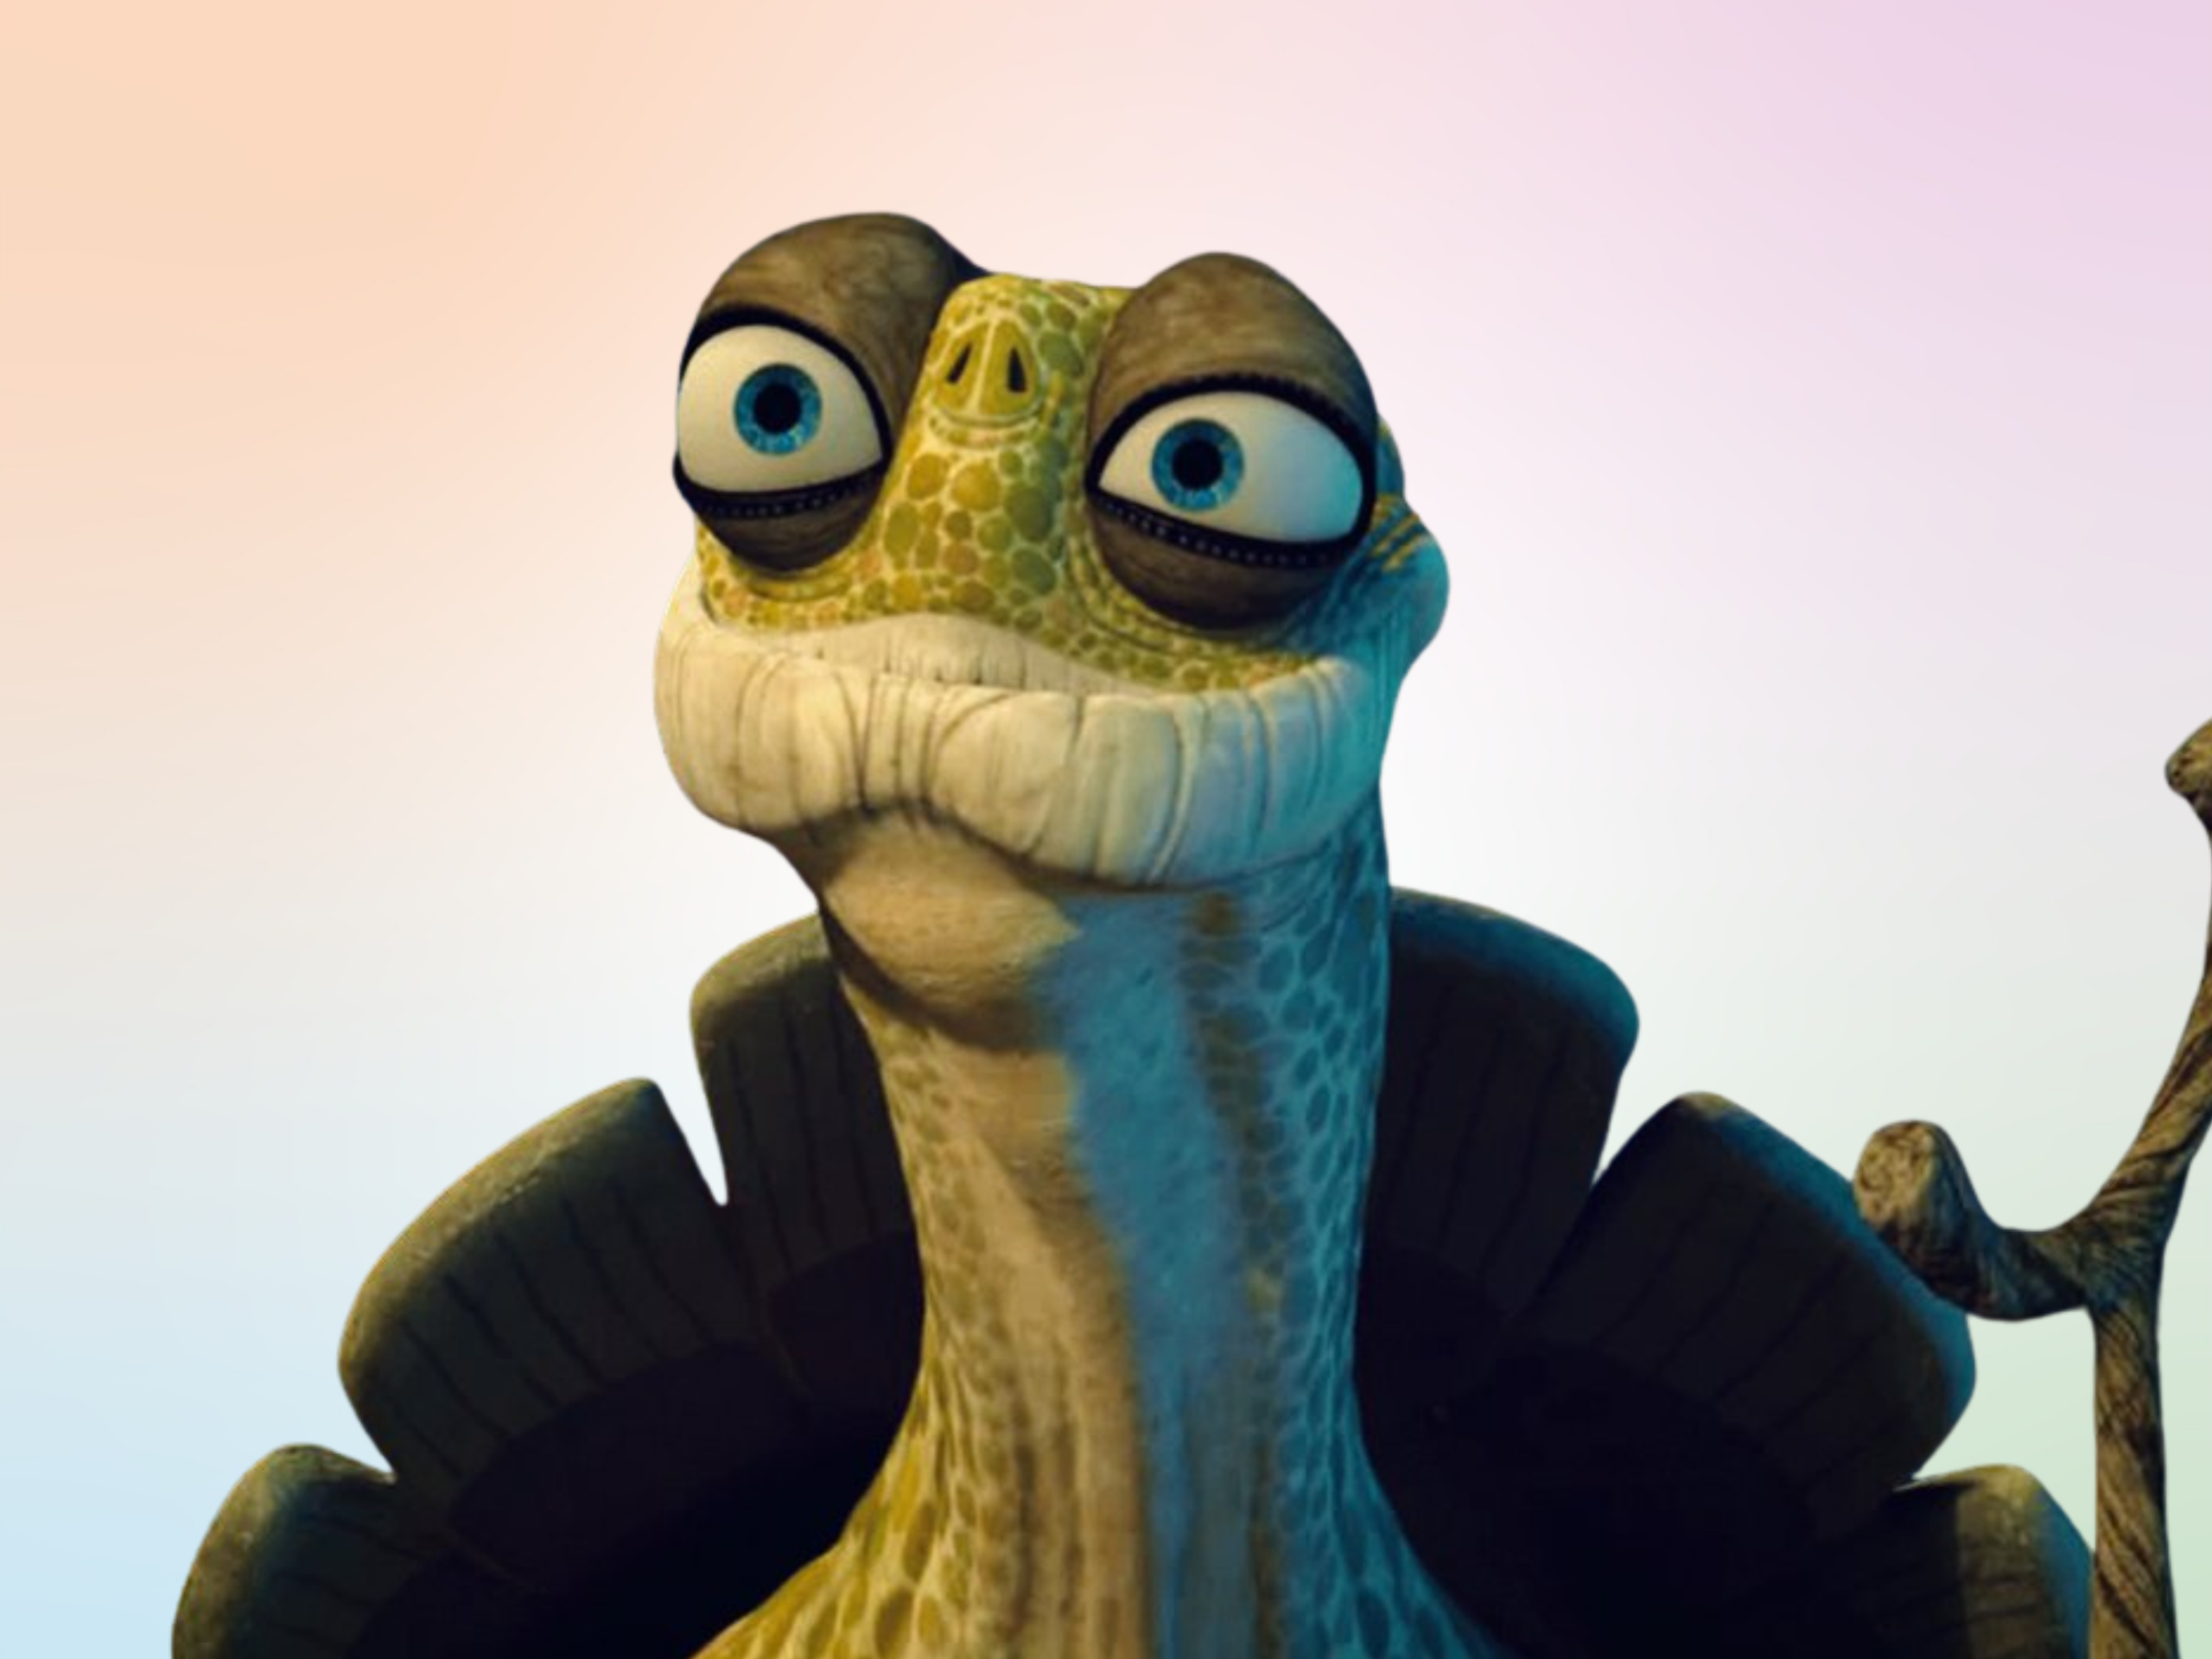
\includegraphics[width=0.5\textwidth]{rysunek1.png}
        \caption{Oogway.}
        \label{fig:rysunek1.png}
    \end{figure}
\end{frame}

\begin{frame}{Rysunki}
    \begin{figure}[h]
        \centering
        \begin{minipage}{0.45\textwidth}
            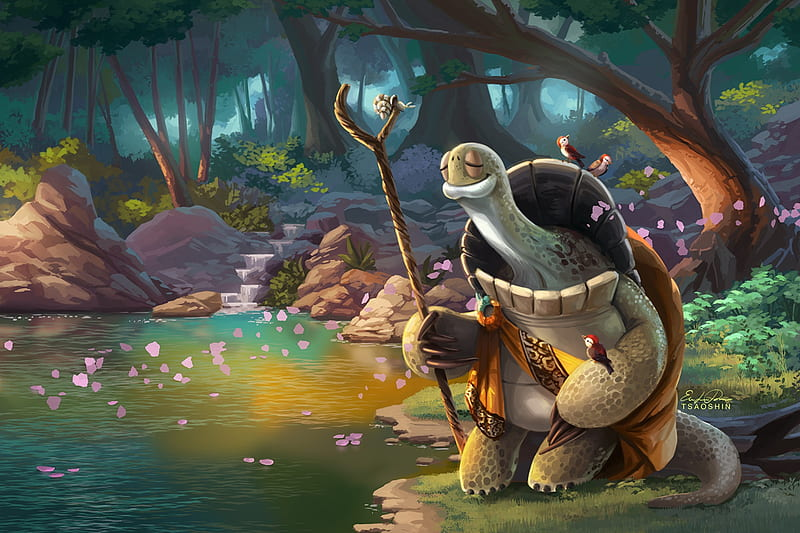
\includegraphics[width=\textwidth]{rysunek2.png}
            \caption{Oogway.}
        \end{minipage}
        \hfill
        \begin{minipage}{0.45\textwidth}
            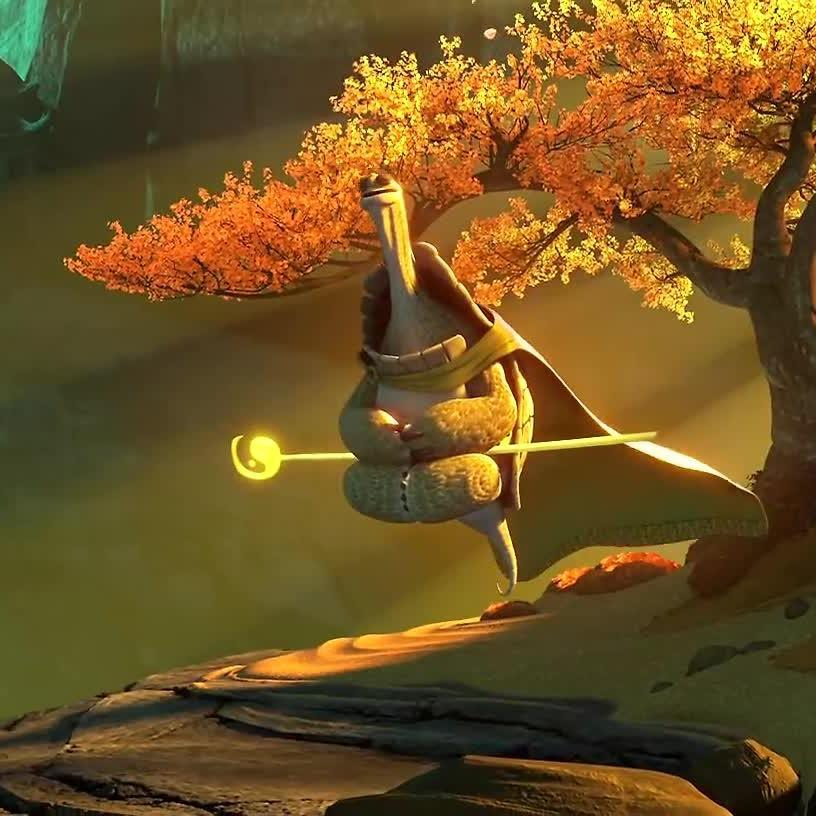
\includegraphics[width=\textwidth]{rysunek3.png}
            \caption{Oogway.}
        \end{minipage}
    \end{figure}
\end{frame}

\section{Tabela}
\begin{frame}{Tabela}
    \begin{table}[h]
        \centering
        \begin{tabular}{|c|c|}
            \hline
            Kolumna 1 & Kolumna 2 \\
            \hline
            Wartość 1 & Wartość 2 \\
            \hline
            Wartość 3 & Wartość 4 \\
            \hline
        \end{tabular}
        \caption{Tabela odnosząca się do tekstu.}
        \label{tab:tabela1}
    \end{table}
\end{frame}

\section{Elementy Dynamiczne}
\begin{frame}{Elementy Dynamiczne}
    \begin{itemize}
        \item<1-> Pierwszy punkt
        \item<2-> Drugi punkt
        \item<3-> Trzeci punkt
    \end{itemize}
\end{frame}

\section{Odwołania}
\begin{frame}{Odwołania}
    Odniesienie do Rysunku \ref{fig:rysunek1.png}, Tabeli \ref{tab:tabela1}, oraz równania (1).
\end{frame}

\section{Podsumowanie}
\begin{frame}{Podsumowanie}
    \lipsum[16]
\end{frame}

\begin{frame}{Bibliografia}
    \begin{thebibliography}{9}
        \bibitem{autor1} Autor Nieznany. \emph{Eeeeei}. Operon, 2003
        \bibitem{autor2} Jar Jar Binks. \emph{Jedi}. Czarnekowe, 5002 BC
    \end{thebibliography}
\end{frame}

\end{document}